\chapter{Design Intuition for Wireless Sensor Power Supplies}
\label{chap:intuition}

%There is a rift between industry and research in the way that indoor wireless sensors are powered. Industry has largely eschewed energy harvesting methods, opting instead for the reliability offered by high-density non-rechargeable batteries. 
%Conversely, energy-harvesting is extremely popular for research systems, which have largely abandoned the use of non-rechargeable cells in the pursuit of building systems with indefinite lifetimes. 
%Given this disparity, it is obvious that there is a lack of clarity regarding how wireless sensors should be powered to enable various applications. 
Wireless power supplies are the result of a multi-dimensional design space exploration.
While certain design decisions are straightforward, like the choice to use a certain type of harvester to suit an application environment, some design points are more difficult to determine. 
Harvesting and storage technologies are often difficult to directly compare, and it is sometimes difficult to determine the sizing of these elements in order to satisfy the constraints of an application. 
Many times, the type and size of harvesters, batteries, or capacitors are chosen arbitrarily~\cite{hamiltoniot}, or are chosen to make the design minimally feasible~\cite{yervaGrafting12,debruin2013monjolo,hesterFlicker17,afanasov2020battery}.

The goal of this chapter is to provide high-level guidance for navigating the design space of wireless sensor power supplies. 
This chapter seeks to formalize the the application requirements that were discussed in 
\cref{sec:background:background_reqs}.
Using these requirements, this chapter provides guidance to designers for when energy harvesting is a beneficial technique for energy income instead of, or in addition to, a non-rechargeable storage, how prospective income and workloads drive component types and sizing, and if energy-harvesting is utilized, what techniques are required to ensure a minimum useful operation or what is required to capture sufficient energy to maximize system availability. 
To limit scope to a manageable size, 
this chapter, along with the those following, focus exclusively on indoor photovoltaic energy harvesting.
This is because in the conditions of the majority of human-occupied indoor locations, photovoltaic harvesting offers an order of magnitude more energy than other methods.
Despite this focus, similar explorations can be made with other harvesting methods.

\section{Energy Income}
A wireless sensor must source energy from somewhere. 
Energy-harvesting has the potential to supply energy indefinitely. However, harvested energy is often unreliable and unpredictable, and instantaneous power delivery is limited. 
Conversely, primary-only systems have a limited amount of energy, but can use that energy at any rate they please, within the power limits of the battery. 
Because of these differences, it can be difficult to directly compare their performance and determine at what scale and in which conditions harvesting, energy preallocation, or a hybrid of the two, is the preferable power source strategy for any given application.
This section begins with a description of constraints for properly sizing components to ensure a sufficient lifetime and energy income. 
Next, it provides a method of comparison of energy capture potential between harvesting and preallocation methods.
The constraints and relations defined and explored in the following section can be used to estimate proper harvester and battery selection to achieve application requirements.

\subsection{Sizing}
Regardless of how a sensor is powered, it must receive sufficient energy at the right times to continuously and reliably operate.
Assuming that the average power required to drive an application is known at design time, it is relatively straightforward to determine the correct size of a battery to achieve an expected lifetime, or a photovoltaic panel to achieve an average power income.
%The improvement in energy density of batteries and the efficiency of energy harvesting sources has not improved at the same rate as the energy efficiency of CMOS and low power radio technology.
%Barring any transformative improvements in energy storage, energy income is primarily dependent on the volume or area available for a battery or harvester, respectively. 
Usually battery capacity is expressed as accumulated charge in terms of \si{\milli\Ah}.
If the nominal voltage of the battery is known, it can be used to estimate lifetime given a battery's capacity and intended workload.

\begin{equation} \label{eqn:intuition:energy_battery_estimation}
   E_b = U C
\end{equation}
\begin{equation} \label{eqn:intuition:power_battery_estimation}
   P_b = \frac{U C}{T} 
\end{equation}
%\begin{equation}
%   T \approx \frac{U*C}{P_{w}}
%\end{equation}

\noindent 
\Cref{eqn:intuition:energy_battery_estimation} describes the energy contained in a battery of capacity $C$ and a nominal voltage $U$. 
Assuming a desired lifetime $T$, \cref{eqn:intuition:power_battery_estimation} describes the maximum achievable average power supplied by such a battery. 
Likewise, the average power provided by a photovoltaic of area $A$ is described by \cref{eqn:intuition:p_power}. 

\begin{equation} \label{eqn:intuition:p_power}
P_h = \eta E_e A 
\end{equation}

\noindent 
Where 
$\eta$ denotes the efficiency of the photovoltaic, and is often between 18 and 20\%. 
The average energetic spectrial irradiance, $E_e$, is generally between 10 and 100\si{\micro\watt\per\centi\meter\squared} for photovoltaics in indoor conditions~\cite{yervaGrafting12,gorlatova2013networking}. 
Given an average workload power ($P_w$) and a desired lifetime $T$, 
\cref{eqn:intuition:battery_capacity,eqn:intuition:panel_size}
describe the necessary battery capacity and solar cell size.

\begin{equation} \label{eqn:intuition:battery_capacity}
    C \geq \frac{P_w T}{U}
\end{equation}
\begin{equation} \label{eqn:intuition:panel_size}
    A \geq \frac{\eta E_e}{P_w}
\end{equation}

For some applications, it is obvious when utilizing energy harvesting is a better design choice over a battery. 
Such is the case with Zebranet collars~\cite{juang2002energy}. Powering the collar would require a large and heavy battery, beyond the weight constraints of application, and would only power the system for 5 days, far below the lifetime goal of a year or more of operation.
In other cases, it is much more difficult to determine which method is appropriate.
This is especially apparent in environments where available harvestable energy is limited, like indoor environments. 


\subsection{Preallocation versus Harvesting}
In many cases where potential harvestable energy is limited, it is difficult to determine whether energy preallocation or harvesting is the most suitable technique.
It is very difficult to directly compare these methods, as the power and energy supplied by either option is dependent on many factors, including the availability, variance, and magnitude of available harvestable energy, the size of the battery or harvester, and the expected sensor workload. 
%The most important metrics for consideration are the power and energy supplied by battery preallocation or energy harvesting.
%Energy income defines both the lifetime of a sensor, as well as a maximum supportable power available for a workload.
Prior work has attempted to approach a comparison of non-rechargeable energy storage and energy harvesting by comparing the expected average power supplied by either option. 
They simplify the problem by considering a theoretical cubic sensor of volume $V = L^3$, 
with the assumption that the entire cubic sensor volume is dominated by a lithium primary battery, or the entire area of one $A = L^2$ face is dominated by a photovoltaic panel~\cite{yervaGrafting12}.
The authors compare the power provided by the battery cube, with that of the photovoltaic square, over the shelf-life of the battery. 
%concluding that as sensors continue to reduce in size, they will derive more benefit from harvesting over battery preallocation. 

For this analysis, \cref{eqn:intuition:energy_battery_estimation} is not as useful for direct comparisons. 
%for comparing battery energy capacity with photovoltaic energy capture.
A more appropriate method utilizes volumetric energy density.
Battery energy capacity ($E_b$) can be estimated based on the volume of the battery ($V$) and its volumetric energy density ($\rho$).
While $\rho$ varies depending on the specific battery chemistry, size, and packaging, lithium primary batteries usually provide on the order of 800\si[per-mode=symbol]{\milli\Wh\per\cm\cubed}~\cite{tuna2016energy}. The maximum average power ($P_b$) provided by the battery can be calculated with a desired lifetime ($T$). 

\begin{equation} \label{eqn:intuition:b_energy}
E_b = \rho V 
\end{equation}
\begin{equation} \label{eqn:intuition:b_power}
P_b = \frac{\rho V}{T}
\end{equation}
%The volume of a sensor occupying a rectangular prism of dimensions $L$ length, $W$ width, and $H$ height is given by the following equation.
%
%\begin{equation}
%    V = L * W * H
%\end{equation}
%
%\noindent For an energy harvesting sensor, the side with the largest surface area represents the area available for harvesting with a photovoltaic. This area is represented by the following equation.
%
%\begin{equation}
%   A = L * W 
%\end{equation}
%
%Assuming that an application's power requirements are known before design, the the proper sizing of a battery and photovoltaic can be determined. 
%The energy and power stored in a battery of volume $V$ are described by the following relations:
%
%
%\noindent Where the energy density of the battery is $\rho$ 
%and $T$ is the lifetime of the battery.

\placefigure{fig:intuition:eh_worth_it}

\noindent When considering \cref{eqn:intuition:b_energy,eqn:intuition:b_power}, the authors use a more conservative 653\si[per-mode=symbol]{\milli\Wh\per\cm\cubed} for $\rho$, 
and assume a 7 year lifetime based on shelf-life. They use this lifetime in order to calculate the maximum power that a primary cell can provide over this period~\cite{yervaGrafting12}.
This assumption for battery lifetime is very conservative, as it considers a primary battery entirely empty or unusable after its reported shelf-life.
Assuming a static lifetime also ignores the impact of a sensor's workload power requirements on battery longevity.
Primary battery shelf-life is often poorly defined and understood. While some take shelf-life to mean a battery is expired and not usable after this time, shelf-life actually represents a manufacturer guarantee that a cell will retain a majority of its capacity over the shelf-life period. 
A 10 year shelf-life is common for lithium metal primary batteries~\cite{primary2032,primarycr123a,energizerAppMan}.
Energizer claims that their lithium metal primary batteries experience a self-discharge rate of 1\% per year at room temperature and humidity. This corresponds to 90\% remaining capacity at the end of their listed shelf-life period~\cite{energizerAppMan}.
A lithium battery can hardly be considered empty after its shelf-life has expired.
A more accurate estimation for battery lifetime is:

\begin{equation}
\label{eq:intuition:battery_life}
T = \frac{\rho L^3}{P_w + P_l}
\end{equation}

\noindent Where $P_w$ is the average power required to drive a sensor workload, and $P_l$ is the self-discharge power of the battery. 
Any aging effects other than self-discharge are unpredictable and not considered here. 
With this new definition of battery lifetime, the comparison of power is not as useful a metric, as workload power provided by the battery ($P_w$) is independent of the battery capacity. 
The power provided by a battery \textit{is} technically limited by its maximum rated load current, which is often related to its capacity. 
However, this limit is not usually relevant when considering low power operation.
Conversely, the power provided by an energy harvester is unrelated to the requisite workload power at all, and is incomparable with that of an on-demand preallocated power source.
Instead of power, the energy provided to a workload by a primary cell and the energy captured by a similarly sized photovoltaic over the course of the lifetime of the primary cell are directly comparable.
The energy captured by a photovoltaic over a time period $T$ is represented by \cref{eqn:intuition:p_energy}.
The authors of \cite{yervaGrafting12} assume the lower end of irradiance to provide a conservative estimate, but ignore photovoltaic efficiency $\eta$. This results in an overestimation of harvestable power and energy.
This analysis assumes a conservative photovoltaic efficiency of 17\%.
\Cref{eqn:intuition:p_power,eqn:intuition:p_energy} are more realistic representations of photovoltaic power and energy. 

\begin{equation} \label{eqn:intuition:p_energy}
E_h = \eta E_e A T 
\end{equation}


\placefigure{fig:intuition:eh_worth_it_nano}

With these relations, it is possible to calculate the energy contained in a battery of size $L^3$, the lifetime of that battery given a workload power $P_w$, and the energy captured by a photovoltaic panel of size $L^2$ over the lifetime of the similarly sized battery.
This is visually presented in \cref{fig:intuition:eh_worth_it}, 
an updated energy-harvesting reality check~\cite{yervaGrafting12}. 
This figure compares the preallocated energy provided by a battery with that of the potential harvestable solar energy over the same time period. 
Both battery and harvester energy are driven by the same dimension $L$. 
The energy offered by a battery is represented by the blue line, and increases with $L^3$.
This energy, coupled with power requirements of different workloads, define the lifetime of of the battery ($T$).
The other lines correspond to the energy captured over $T$ via a photovoltaic panel of area $L^2$ in different average lighting and workload conditions.
The two different workloads are represented by the orange (average 25\si{\micro\watt}) and red (100\si{\micro\watt}) lines.
The extents of average indoor photovoltaic harvesting are represented by dashed 
(10\si[per-mode=symbol]{\micro\watt\per\centi\meter\squared}) and solid 
(100\si[per-mode=symbol]{\micro\watt\per\centi\meter\squared}) lines. 
The point at which the harvesting lines (orange, red) cross the battery line (blue) indicate the size at which a solar panel of size $L^2$ will harvest the same amount of energy provided by a battery of size $L^3$ over the lifetime ($T$) of the battery. 
These crossing points also indicate the size at which harvesting collects sufficient average power to drive its intended workload, approaching energy neutral operation.
For appropriate workloads and lighting conditions, the crossing points suggest that a sensor with a driving dimension larger than 4\si{\centi\meter} will be able to harvest more energy than is contained in a similarly sized battery over its lifetime.


The same analysis can be done for designs that scale down in both size and power. Millimeter-scale systems like the Michigan Micro Mote occupies 1\si{\milli\meter\squared} and requires on the order of 100s of \si{\nano\watt} to power its workload~\cite{lee2013modular}.
\Cref{fig:intuition:eh_worth_it_nano} is a reconfigured analysis, tuned for \si{\nano\watt} workloads and millimeter-scale systems. The same dark blue line represents the energy preallocated with a lithium battery of size $L^2$. The green lines represent a 100\si{\nano\watt} average workload, and the teal lines represent 25\si{\nano\watt} workload. This figure considers the same lighting conditions as the previous figure.
Likewise, there are sensor sizes where workloads and lighting conditions result in a sensor that will be able to collect more energy over time with energy harvesting than can be preallocated with a battery.
This reaffirms the design decisions made by the designers of many of the millimeter-scale systems, who chose to utilize energy harvesting to prolong the lifetime beyond that of a non-rechargeable battery. 

\placefigure{fig:intuition:compound}

\subsection{Hybrid}
At the crossing points in \cref{fig:intuition:eh_worth_it,fig:intuition:eh_worth_it_nano}, the benefits of energy harvesting are compounded when considering that energy capture will continue indefinitely, beyond that of the lifetime of a battery.
However, this energy is not guaranteed to be supplied at times when the system requires it, even when harvesting supplies enough on average to match that of workload. This reality has the potential to result in unexpected system outages and system resets.
To ensure that a system always has sufficient energy available, a hybrid system can utilize energy harvesting with a backup preallocated energy storage. 
This section considers an cubic sensor with length $L$, with a non-rechargeable battery comprising a volume of $L^3$, and a harvester taking up one $L^2$ side of the cube face.
A hybrid system can operate even in the absence any ambient or accumulated harvestable energy. A hybrid system will possess a finite lifetime, but will have guaranteed reliability during its lifetime. 
This lifetime primarily depends on the disparity between its intended workload and the availability of harvestable energy.
This disparity can be expressed by \cref{eqn:intuition:p_total}. 
If the average power supplied by a photovoltaic harvester is sufficient to drive the intended workload, the total drain, $P_t$, on the battery is equal to its self-discharge power, $P_l$. 
If the photovoltaic does not harvest sufficient power for the workload, the battery is drained at an average rate of the difference, plus the battery self-discharge.
Given this new definition of battery drain power, the lifetime of its battery now resembles \cref{eqn:intuition:compound}.
\begin{equation} \label{eqn:intuition:p_total}
    P_t = 
    \begin{cases}
        P_l & \text{if $P_w < P_h$} \\
        P_w - P_h + P_l & \text{if $P_w \geq P_h$}
    \end{cases}
\end{equation}
\begin{equation} \label{eqn:intuition:compound}
T = \frac{\rho L^3}{P_t}
\end{equation}
If the amount of average harvestable power is greater than required for a sensor workload, the lifetime of a hybrid system is compounded. 
The additional energy captured lengthens the lifetime of the system, and the longer lifetime allows for additional energy capture. 
\Cref{fig:intuition:compound} explores this relationship visually, using the same workloads, lighting conditions, and visual scale and line types as \cref{fig:intuition:eh_worth_it}. The additional energy capture results in the battery line crossing points shifting to the left, meaning that in a hybrid system a smaller harvester and battery are required to capture the same amount of energy as that provided by a battery when compared to a harvester-only system.
For a hybrid system, these crossing points represent a design point that is able to harvest the same amount of energy as it has preallocated, in effect providing twice the energy as a battery-only system of the same dimensions.
As the size of the system increases beyond the size at which the harvesting lines and battery line cross, the energy supplied by harvesting begins to approach a vertical line. 
This represents the size at which the average income from harvesting is sufficient to power the workload. 
When harvesting can sustain the system indefinitely, the backup primary battery is infrequently or never utilized, and its lifetime is only limited by its self discharge.
These locations where the harvesting energy lines approach verticality represent the ideal sizing for a hybrid system given an intended workload and lighting conditions.
This ideal sizing results in a harvester large enough to capture enough average power to results in energy neutrality, where the system harvests enough energy to sustain its operation.

\subsection{Limitations}

The above analysis is a simplified view of a complex reality.
The analysis assumes that a sensors workload and income can be treated as static averages.
While a case can be made that on a timescale of hours to days, for many applications a sensor's workload power can be consolidated into an average. 
The same assumption can not easily be made for energy income.
For example, lighting conditions are often both diurnal and seasonal, meaning that a daily or even weekly average income from a photovoltaic will vary significantly over the course of a day or year depending on the angle and intensity of sunlight, or the occupancy and activation of artificial lighting.
It is a common challenge for energy harvesting systems to continue operating when there is insufficient harvestable energy.
For this problem, the reliability and uptime benefits of adding non-rechargeable backup energy storage in a hybrid sensor are not highlighted in this analysis.

For simplicity's sake, the analysis of this section also assumes the whole sensor volume is available for energy storage, and a whole face is available for energy harvesting.
This assumption breaks down when considering sensors and PCB elements that require substantial volume, such as a PIR sensor, or a sensor that can not be covered by a harvesting element, such as an image sensor or light sensor.
However, the relationship to energy capacity and harvesting capability are directly and linearly related to volume and area respectively. The general conclusions should hold, even if some percentage of the volume and area of a sensor are occupied by elements other than energy storage or harvesting. 

The above analysis also does not consider the effect of rechargeable energy capacity on energy income from harvesting. 
The analysis assumes an ideal rechargeable energy storage with limitless storage.
In reality, energy storage elements are far from limitless or ideal.
A small energy capacity will fill up often, requiring shunting of any additional harvested energy. 
By shunting, or wasting this energy, a system with insufficient capacity will effectively reduce the average energy income power available to it. \Cref{chap:intuition:feasibility,chap:intuition:capacity} explore the effect of capacity in further detail.

The analysis of this section also does not consider the effects of miniaturization, especially as components approach the scale of millimeters and their packaging begins to dominate their volume. As batteries reduce in size, the proportion of volume available for energy storage versus the volume taken by packaging decreases, resulting in less energy density. This analysis assumes a static energy density for lithium primary cells, when in reality the density would also decrease as the size of the battery decreases. Similarly, harvesting elements experience less surface area for the actual harvester versus area required to hold and provide electrical connections at smaller scales.
System designers seeking to build extremely small devices will have to consider additional factors when considering element sizing.
Despite these limitations, the analysis of this chapter has enough basis to serve as a guiding rule-of-thumb when considering methods for energy income as well as component sizing requirements for various applications. 



%data type quanta vs rate
%reporting rate periodic, reactive

%Given a set of application requirements, what are the constraints on the power supply?
%\begin{enumerate}
%%\item Mobile or static?
%\item What size does it have to be?
%
%    
%    $V_{primary} + V_{secondary} < V_{max}$
%    
%\item What are the average power requirements, and what is the largest atomic energy quanta?
%    
%    $P_{avg, period} = \frac{P_{sleep} * (T_{period} - T_{work}) + P_{work} * T_{work}}{T_{period}}$
%    
%    Assuming a Poisson distribution over a period $T$:
%    
%    $P_{avg, reactive} = \frac{P_{sleep} * (T - \lambda * T_{work}) + \lambda * P_{work} * T_{work}}{T}$ 
%   
%    $P_{avg, intermittent} = P_{harvest}$
%    
%    $E_{work} = \sum\limits_{e_i\in E} e_i$
%    
%    $E_{atomic} = \max{E}$
%    
%    $E_{comms} \in E$
%    
%    
%\item What are the energy storage and lifetime requirements?
%    
%    $E_{primary} < \rho_{primary} * V_{primary}$
%    
%    $E_{secondary} < \rho_{secondary} * V_{secondary}$
%    
%    $E_{secondary} > E_{atomic}$
%    
%    How to express size of secondary mathematically?
%    Energy capacity represents a moving capped sum, is this like a moving average? What is the smallest window that gives us the most return on energy capture?
%    At some point, a large enough window allows us to consider the average of harvestable energy, instead of the actual distribution. What is that size?
%    
%    Given a time series vectors of harvestable and consumed energy of length $N$ seconds:
%    
%    $P_{trace} = [e_1, e_2, \dots, e_N]$
%    
%    $P_{work} =  [w_1, w_2, \dots, w_N]$
%     
%    at any time $i$, the cumulative energy will be
%    
%    $ y_0 = \begin{cases} 
%        0         & \text{if $e_i - w_i < 0$} \\
%        e_i - w_i & \text{if $e_i - w_i > 0$} \\
%        E_{secondary} & \text{if $e_i - w_i > E_{secondary}$}
%    \end{cases}$
%    
%    $ y_i = \begin{cases} 
%        0             & \text{if $y_{i-1} + e_i - w_i < 0$} \\
%        y_{i-1} + e_i - w_i     & \text{if $y_{i-1} + e_i - w_i > 0$} \\
%        E_{secondary} & \text{if $y_{i-1} + e_i - w_i > E_{secondary}$}
%    \end{cases}$
%    
%    usable workload energy:
%     
%    $ z_i = \begin{cases} 
%        0             & \text{if $y_{i} \leq 0$} \\
%        w_i           & \text{if $y_{i} \geq w_{i}$} \\
%    \end{cases}$
%    
%     
%    %for an ideal limitless storage:
%    % 
%    %$ x_0 = \begin{cases} 
%    %    0         & \text{if $e_i - w_i < 0$} \\
%    %    e_i - w_i & \text{if $e_i - w_i > 0$} \\
%    %\end{cases}$
%    %
%    %$ x_i = \begin{cases} 
%    %    0             & \text{if $x_{i-1} + e_i - w_i < 0$} \\
%    %    x_{i-1} + e_i - w_i     & \text{if $x_{i-1} + e_i - w_i > 0$} \\
%    %\end{cases}$
%    %
%    %Unused energy:
%    %
%    %$ w_i = x_i - y_i$
%    %
%    %$ E_{unused} = \sum_{i=0}^N w_i$
%    
%    Assuming all energy can be harvested:    
%
%    $E_{h, total} = P_{harvest} * T_{life}$
%  
%    actual:
%   
%    $E_{h, actual} = \sum\limits_{z_i\in E} z_i$
%    
%    $P_{h, actual} = E_{h, actual} / T_{life}$
%    
%    
%   
%    $E_{total} = E_{primary} + E_{h} $
%    
%    $E_{total} \ge P_{avg} * T_{life}$
%    
%    $T_{life} = \frac{E_{total}}{P_{avg}}$
%    
%    
%\item How does the average power requirements compare to available harvestable power? 
%    
%    Energy neutrality:
%    
%    $P_{h} \ge P_{avg}$ 
%    
%\item What are the reliability requirements?
%\item What are the latency requirements?
%\end{enumerate}


\section{Harvesting Feasibility and Reliability}
\label{chap:intuition:feasibility}
From the previous section, it is obvious that the availability and magnitude of harvested energy directly impacts the energy income of an energy harvesting system. 
What is perhaps not as obvious is that the energy capacity of the rechargeable storage element used to capture harvested energy also impacts the energy income of the system.
The magnitude of available harvested power, an application workload, and the size of an energy buffer determine whether a design is minimally feasible, and where the design lies on a gradient of metrics like reliability and availability.
This section seeks to illustrate this relationship and define operating regimes based on harvesting energy income and energy storage.
This analysis will provide guidance regarding whether a design is feasible and whether it requires intermittent techniques to ensure operation and forward progress.

%Depending on the design point, a design can offer minimal feasibility, 
%We seek to illustrate the design space for energy-harvesting sensors in two
%ways. The first defines an energy-harvesting sensor framework to examine
%when designs are feasible and when they require intermittent techniques to make meaningful forward progress.
%The second examines dynamic income energy and device behavior through numerical
%modeling and simulation.  The framework is based on three key metrics:
%harvested energy income, workload, and capacity.
\placefigure{fig:intuition:framework}

\subsection{Design Regimes}
\label{sec:framework:regime}
\Cref{fig:intuition:framework} splits the design space into four main regimes: always on,
infeasible, checkpointing required, and no intermittent techniques required.
These regimes and their constraints are explained in more detail below. 

\subsubsection{Always On} 
If the energy harvester reliably supplies a sensor with
more power than the maximum instantaneous power it will ever draw, then the power supply does not need significant
energy capacity to remain operational. 
This design point constraint is defined by \cref{eqn:intuition:always_on}.
\begin{equation}
    \label{eqn:intuition:always_on}
    P_{w,max} \leq P_{h,avg}
\end{equation}
Where $P_{w,max}$ represents the maximum instantaneous power required by a sensor workload, and $P_{h_avg}$ is the average harvesting income. Additionally, $P_h$ must also have minimum variance (i.e. $Var(P_h) \approx 0$), on the order of normal power ripples handled by power supply bypass capacitors.
If the harvesting power has significant variance or frequent outages, 
then a sensor must have some ability to buffer energy to use when its
instantaneous operating power exceeds that of the harvester input power.
This green region of \cref{fig:intuition:framework} represents design points that have sufficient income power to be \textbf{Always On}.

\subsubsection{Infeasible} 
If the energy harvester supplies less average power than
the system self discharge and leakage, the system will never be able to charge its energy buffer.
Leakage can exist in a system via component quiescent currents, battery or capacity self-discharge, and parasitic resistance that is not eliminated when the system is powered off. 
The constraint on minimum harvesting income and system leakage is described by \cref{eqn:intuition:leakage}.
\begin{equation}
    \label{eqn:intuition:leakage}
    P_{h,avg} > P_l
\end{equation}
Where $P_l$ is the total system leakage in a powered off state.
Similarly, if the energy buffer capacity is less than the
energy required to perform a workload's largest atomic operation, 
%with energy harvested
%during the operation itself, 
then that operation will not have enough energy to
complete.
The total energy required for a single iteration of a sensor workload can be simplified to a finite set of $n$ operations. %that are executed periodically or in response to an event. 
%The energy required to perform one iteration of a workload is the sum of the energy required for each of the $n$ individual atomic operations that make up the workload task.
The set $E_a$ of energy required for each atomic operation in a workload is described by \cref{eqn:intuition:atomic_set}.
%The sum of $E_{a}$ represents the amount of energy required for one iteration of a workload $E_w$, described by 
%\cref{eqn:intuition:workload_sum}.
\begin{equation} \label{eqn:intuition:atomic_set}
    E_{a} = \{e_{i}\}_{i=0}^n
\end{equation}
Each individual $e_{i}$ represents the energy required for a single atomic operation such as sampling a sensor,
sending a radio packet, a processor power on reset, and performing a checkpoint.
The energy capacity ($E_{capacity}$) of a system must be equal to or greater than the largest atomic operation ($max E_a$). This constraint is described by  \cref{eqn:intuition:atomic}.
\begin{equation}
    \label{eqn:intuition:atomic}
    E_{capacity} \geq \max E_a
\end{equation}
Designs that do not have sufficient income, or have insufficient energy capacity to perform a necessary operation will never make forward progress and are
therefore infeasible.
The red regions of \cref{fig:intuition:framework} represent design points that are \textbf{Infeasible}.

\subsubsection{State Preservation Required}
If the energy capacity of the energy buffer 
is sufficient to perform the largest atomic operation as in \cref{eqn:intuition:atomic}, but
not enough to complete
the entire set of operations in the workload, $E_a$,
then a mechanism for state preservation is required to ensure forward progress over power loss and reboots.
A design requires state preservation techniques if \cref{eqn:intuition:checkpointing} is satisfied.
\begin{equation}
    \label{eqn:intuition:checkpointing}
    \max E_a \leq E_{capacity} < \sum_{e \in E_a} e
\end{equation}
In \cref{fig:intuition:framework} this represents the blue region.  
%composed of multiple, chained
%atomic operations (such as sampling a sensor and then sending a radio packet), then
%a mechanism for saving state and continuing progress on the next reboot
%must be employed.
%\begin{equation} \label{eqn:intuition:workload_sum}
%    E_w = \sum_{i=0}^{n} e_{i} \in E_a
%\end{equation}

\subsubsection{No State Preservation Required} A sensor that has enough harvester
potential and energy capacity to complete a workload's longest non-atomic
operation can operate without checkpointing. Such systems also benefit as
energy devoted to checkpointing can be used for a workload instead.

\subsubsection{Hysteresis Management}
Finally, if a sensor's deep sleep power draw 
is a substantial fraction of the harvester power, as
is the case with Capybara~\cite{colinReconfigurable18}, then it is
beneficial to continue operating until the energy
buffer is depleted, power off, and recharge quickly
rather than stop early and recharge slowly.
Under this scenario, hysteresis management techniques,
such as reconfigurable capacity and federated energy can increase sensor
performance as discussed in \cref{sec:related}.
The utility of hysteresis management is diminished
when the ratio of harvester power to deep sleep power increases.
For sensors that can willfully power off or sleep,
operating thresholds can be controlled, disentangling
capacity and charging hysteresis.
Their deep
sleep power is equal to leakage, and such techniques
will not improve recharge times.

For all systems, these techniques can decrease cold start time
by reducing the capacity that must be charged
to achieve cold start.

This is more beneficial for systems that cold start frequently and
have a higher energy capacity, however,
a higher-capacity energy store also has a lower probability of
needing to cold start. Therefore the benefits of hysteresis management for
cold start with respect to storage capacity are in conflict with their necessity,
and we do not attempt to quantify these subtle nuances in \cref{fig:intuition:framework}.

\subsection{Framework Limitations}
\label{sec:framework:limitations}
This framework makes a couple simplifying assumptions that prevent it from
fully capturing the richness of the design space.\\

\vspace{-6pt}
\noindent
\textbf{Backup Energy Store.}
This framework does not consider the impact of a backup energy store.
%that is pre-charged before the sensor begins operation.
%The simplest way
%to view
A backup energy store can be viewed as the ability to inject additional energy
to the system at arbitrary times,
%move the system
%outside of the regime of requiring checkpoints for very energy intensive operations, or
eliminating the need for checkpointing when there is very low
harvesting potential.

A backup energy store could also contribute in more subtle ways. It could
allow a system to avoid the energy and complexity of checkpointing by
providing just enough energy for a deep sleep mode with state retention rather
than a full power down when the system depletes its stored energy. It could also
cold start energy buffer charging to eliminate the need for reconfigurable
power supplies, or to increase the efficiency of
the energy-harvesting front-end at low voltages.
Finally, in periods of long energy drought, the backup energy store could increase
sensor availability.

While the use of a backup energy store
does constrain the sensor to a finite lifetime,
%especially since current technology favors non-rechargeable, primary-cells as
%backup energy stores,
energy-harvesting can substantially extend these lifetimes under certain harvesting
conditions.\\
%We explore the lifetime of energy-harvesting
%designs with backup energy stores in \cref{sec:primary}.

\vspace{-6pt}
\noindent
\textbf{Constant Harvester Power.}
The framework assumes an energy harvester will supply a constant energy
income, when in reality income is often highly variable. In practice, a sensor
platform both defines the regions of the plot, and occupies a
vertical line which represents the energy storage capacity of the sensor
combined with the range of harvester input powers it might experience. We expect
this line will span multiple regions for most sensors.

However, by ignoring variability, the plot also fails to illustrate key benefits
of capacity under varying energy incomes and workloads. Intuitively,
higher energy buffer capacity can store energy in times of excess and supply
that energy in times of drought. This balancing out of energy income
effectively raises the minimum power supplied by the energy harvester.
Because the extent of this impact is completely dependent on the variability
of the energy income and workload of the sensor, we also develop a numerical simulation to
quantify the impact of capacity
on key metrics including energy utilization, availability and reactivity.

\section{A Case for Capacity}
\label{chap:intuition:capacity}

\begin{definetable}{tab:related}
  \scriptsize
  \begin{threeparttable}
  \centering
  \begin{tabular}{l | c c| c c| c}
      \multirow{2}{*}{Platform} & \multicolumn{2}{c|}{Successful Events\,(\%)}  & \multicolumn{2}{c|}{\parbox{2.5cm}{\centering Long-Running\\Time to Completion Ratio}} & \multirow{2}{*}{Lifetime\,(yrs)}\\
                              & Periodic     & Reactive                     & Average & 95th Percentile & \\
    \hline
    Telos \cite{polastre2005telos}                      & 100   & 100   & 1     & 1     & 8.55\\
    Hamilton \cite{kim2018system}                & 100   & 100   & 1     & 1     & 6.75\\
    BLEES \cite{adkins2015michigan}                     & 100   & 100   & 1     & 1     & 1.11\\
    Gecko \cite{yervaGrafting12}                 & 39.5  & 64.9  & 387   & 981   & $\infty$\,\tnote{g} \\
    Capybara~\cite{colinReconfigurable18}\,\tnote{a}    & 46.3  & 72.8  & 37.6  & 1     & $\infty$\,\tnote{g}\\
    Capybara~\cite{colinReconfigurable18}\,\tnote{b}    & 41.1  & 67.1  & 2730  & 8900 & $\infty$\,\tnote{g}\\
    Flicker \cite{hesterFlicker17}                      & 39.3  & 64.2  & 1307  & 5670 & $\infty$\,\tnote{g}\\
    EnHANTs \cite{margolies2015energy}                  & 79.4  & 96.0  & 1     & 1     & \textemdash\,\tnote{h}\\
    DoubleDip \cite{martin2012doubledip}                & 77.9  & 66.5  & 1     & 1     & \textemdash\,\tnote{h}\\
    \cite{raisigel2010autonomous}                       & 78.4  & 66.9  & 1     & 1     & \textemdash\,\tnote{h}\\
    \textbf{\name}\,\tnote{c}                           & 81.2  & 98.3  & 1     & 1     & \textemdash\,\tnote{i}\\
    \textbf{\name}\,\tnote{d}                           & 100   & 100   & 1     & 1     &  35.8\\
    \textbf{\name}\,\tnote{e}                           & 100   & 100   & 1     & 1     &  30.2\\
    \textbf{\name}\,\tnote{f}                           & 100   & 100   & 1     & 1     &  6.27\\
  \end{tabular}
    \begin{tablenotes}[para]
      \item[a] With capacitors: 400\,\si{\micro\farad} ceramic + 330\,\si{\micro\farad} tantalum + 67.5\,mF supercapacitor.
      \item[b] With capacitors: 300\,\si{\micro\farad} ceramic + 1100\,\si{\micro\farad} tantalum + 7.5\,mF supercapacitor.
      \item[c] No primary-cell.
      \item[d] AA primary-cells like Telos.
      \item[e] CR123A primary-cell like Hamilton.
      \item[f] CR2032 like BLEES.
      \item[g] Lifetimes are theoretically infinite for capacitor-based systems.
      \item[h] Not enough information to predict cycling failure time for theses systems.
      \item[i] Expect cycling failure in 20-50 years, but do not attempt to estimate.
    \end{tablenotes}
  \end{threeparttable}
  \caption{
  \normalfont
      Modeled performance of energy-harvesting systems.
    For each  platform considered, we model the performance of its energy storage
    architecture. Periodic workload and lifetime estimates are based on a 10\,s
    period, and the reactive workload is scaled to
    generate a maximum of 2000 events per hour (3.4\,s average daily period). Generally,
    intermittent systems have significantly worse availability and responsiveness compared to
    battery-only systems and systems that use a secondary-cell. Battery-only
    systems achieve perfect operation, but have finite, sub-decade lifetimes.
    }
\end{definetable}

\begin{definefigure}{fig:intuition:framework}
  \centering
  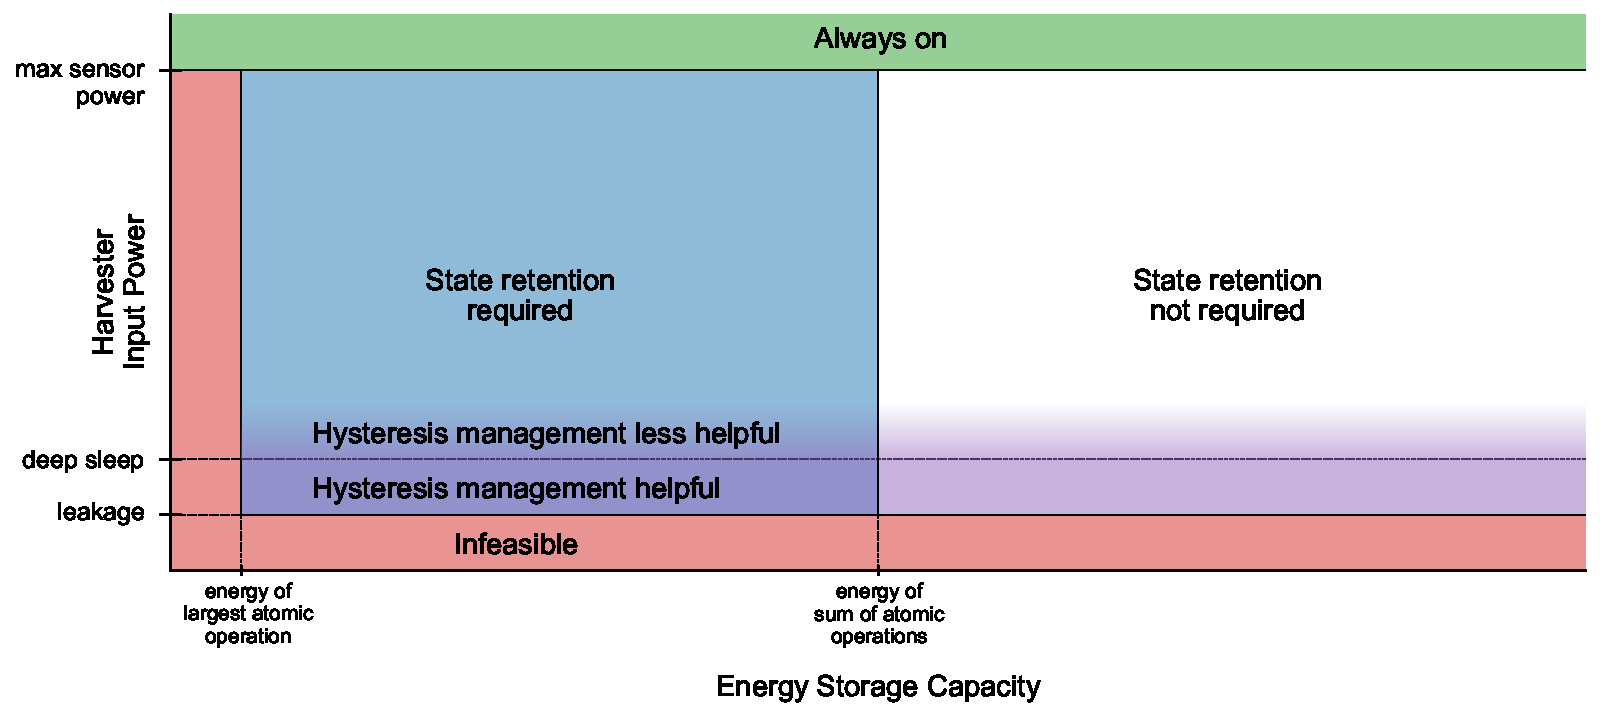
\includegraphics[width=\columnwidth]{figs/capacity/harvesting_framework/framework}
  \caption{
  %energy-harvesting
  %sensors have different capabilities and requirements
  \normalfont Design space for energy-harvesting sensors based on their energy
  income (which we assume is constant for this analysis), energy storage capacity, and workload.
  Workload is represented by the set of atomic operations required by an application, 
  as well as the deep sleep and leakage power.  The plot breaks
  into four regions: {\color{Green}\textit{Always On}} 
  or effectively powered, {\color{BrickRed}\textit{Infeasible}} due to lack of energy storage or
  leakage higher than harvesting rate, feasible but {\color{CornflowerBlue} \textit{Requires State Retention}} 
  to make forward progress, and enough energy storage so that  
  \textit{State Retention is Not Required}. Additionally, sensors which have high
  power when they enter deep sleep before depleting their
  energy buffer may benefit from {\color{DarkOrchid}\textit{Hysteresis Management}} techniques.
  This benefit diminishes with lower sleep currents and higher harvesting potential.
  %With increased capacity, sensors can avoid the complexity of intermittent
  %programming techniques and specialized, reconfigurable power supplies in addition
  %to the other benefits of increased capacity discussed
  %in \cref{sec:store}.
  }
\end{definefigure}


\begin{definefigure}{fig:intuition:eh_worth_it}
  \centering
  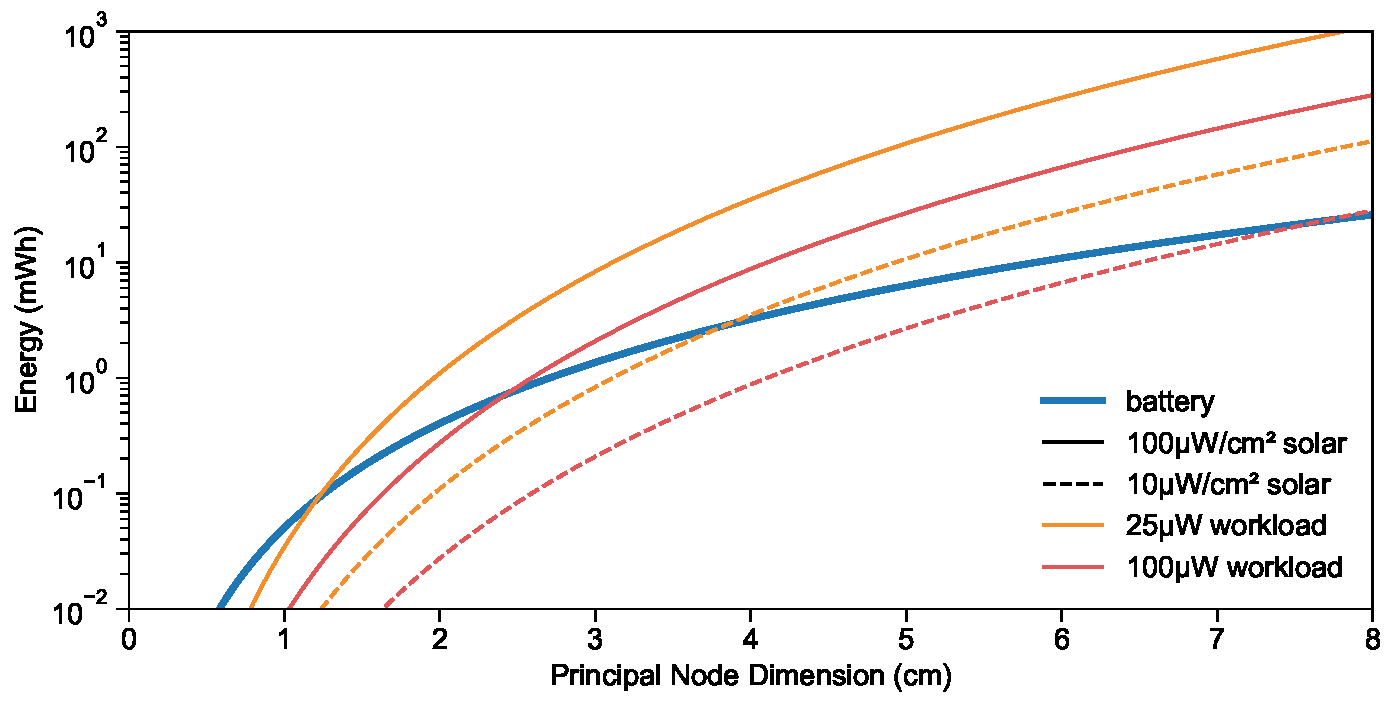
\includegraphics[width=\columnwidth]{figs/is_eh_worth_it_micro.pdf}
  \caption{
  A comparison of preallocated energy and captured energy. Note the logarithmic y-axis scale.
  This figure compares the energy offered by a cubic battery with that of potential harvestable energy captured by a square photovoltaic over the lifetime of the battery. 
  %The lifetime of the battery depends on different workloads, 
  %here represented by the orange (average 25\si{\micro\watt}) and red (100\si{\micro\watt}) lines. 
  %A solar cell accumulates energy over that same lifetime under different harvesting conditions, represented by a solid line 
  %(100\si[per-mode=symbol]{\micro\watt\per\centi\meter\squared}) or dashed line
  %(10\si[per-mode=symbol]{\micro\watt\per\centi\meter\squared}).
  %The point at which the harvesting lines (orange, red) cross the battery line (blue) indicate the size at which a similarly sized photovoltaic will harvest the same amount of energy provided by a similar sized battery over its lifetime. 
  At a sufficient size and in sufficient harvesting conditions, while powering an appropriate workload, solar energy-harvesting can provide more energy over the same time frame as a lithium battery.
  }
\end{definefigure}

\begin{definefigure}{fig:intuition:eh_worth_it_nano}
  \centering
  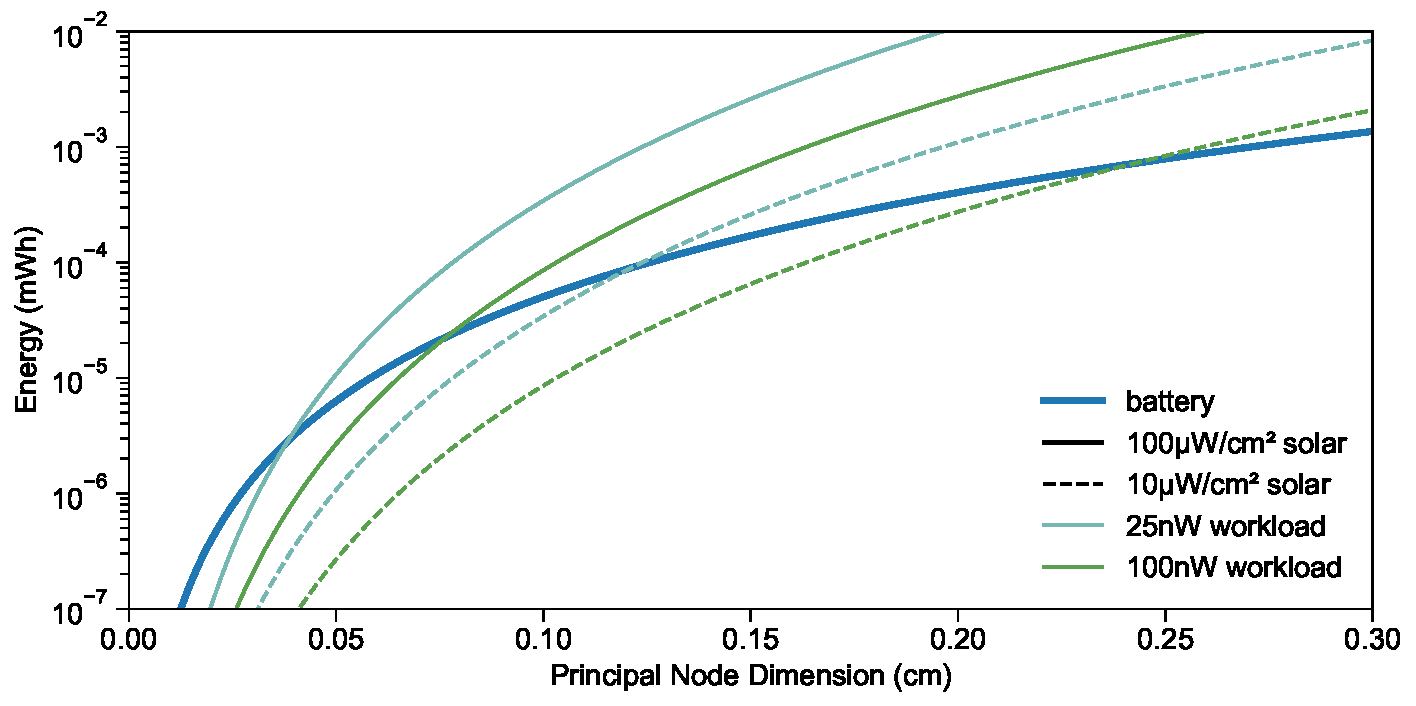
\includegraphics[width=\columnwidth]{figs/is_eh_worth_it_nano.pdf}
  \caption{
  A comparison of preallocated energy and captured energy for \si{\nano\watt} applications. 
  This figure is identical to \cref{fig:intuition:eh_worth_it} except that it considers the \si{\nano\watt} workloads that characterize millimeter-scale systems.
  A principle node dimension on the order of 1-2\si{\milli\meter} is generally sufficient for energy harvesting to collect more energy over a battery, in all but the worst case: a heavier workload with low harvesting potential.
  }
\end{definefigure}


\begin{definefigure}{fig:intuition:compound}
  \centering
  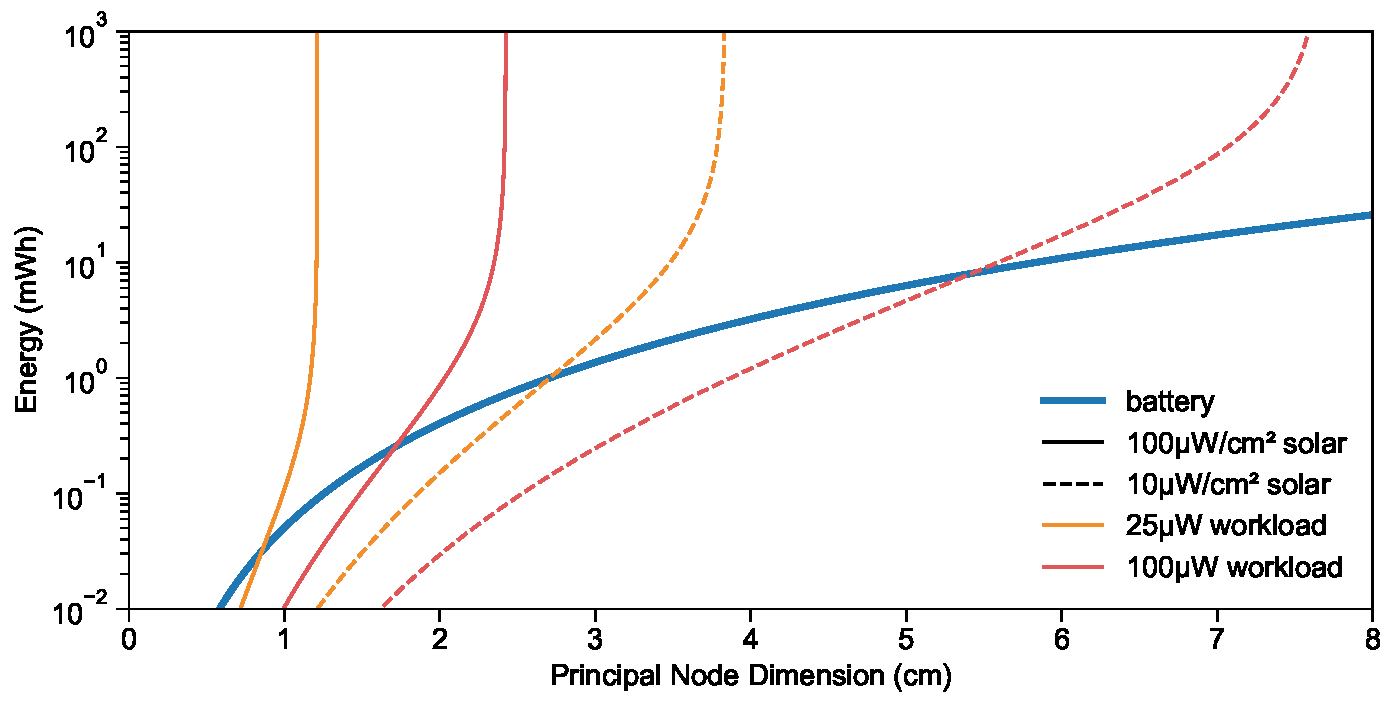
\includegraphics[width=\columnwidth]{figs/is_eh_worth_it_micro_compound.pdf}
  \caption{
    The energy captured by a hybrid system utilizing both harvesting and backup preallocated energy. This figure uses the same scale and line types as \cref{fig:intuition:eh_worth_it}. The addition of energy harvesting to a primary cell system has a compounding effect on lifetime and harvested energy. More harvested energy results in a prolongation of the lifetime of the primary cell. Subsequently, this lifetime extension results in an increase in harvested energy. 
    Because of the increased energy and battery lifetime, the crossing points now shift to the left in the figure, allowing a reduction in volume and area required for a battery and harvester, respectively. 
  }
\end{definefigure}